\documentclass[a4paper,oneside]{article}

\usepackage[frenchb]{babel}
\usepackage[utf8]{inputenc}  
\usepackage{graphicx}
\usepackage{url}
\usepackage{float}
\usepackage{color}
\usepackage{hyperref}
\usepackage{multicol}
\usepackage{latexsym}
\usepackage{amssymb}
\usepackage{wrapfig}

\usepackage{geometry}
\geometry{left=3cm,right=3cm,top=3cm,bottom=2cm}

\title{\huge Proposition de module d'aide à la programmation}
\author{L\'eo \textsc{Baudouin}}

\begin{document}
\maketitle

%----------------------------------------------------------------------

\noindent Pour plus d'informations, contactez moi à l'adresse : 
\href{mailto:baudouin.leo@gmail.com}{\nolinkurl{baudouin.leo @ gmail.com}}.

%----------------------------------------------------------------------

\section{Motivation}

Les étudiants débutant leurs thèses sont souvent libres de choisir de quelle façon ils souhaitent programmer.
Cette trop grande liberté peut être néfaste dans le cadre d'une thèse qui se doit d'être un projet solidement construit et souvent partagé avec d'autres doctorants ou chercheurs.

Ce module a pour but de proposer des outils d'aide à la programmation afin de faciliter le développement des programmes pour les doctorants mais également son partage au sein d'une équipe ou d'un laboratoire.
Les outils présentés sont des standards libres, gratuits et multi-plateformes et sont donc utilisables par tous.

\section{Détails}

\begin{itemize}
\item[\textbf{Cible :}] \'Etudiants utilisant la programmation (informatique, robotique, mathématiques, \dots) 
\item[\textbf{Effectif :}]  24 personnes environ
\item[\textbf{Durée :}]  2 journées
\item[\textbf{Intervenant :}]  1
\item[\textbf{Salle :}] Salle informatique sous Linux (de préférence Ubuntu 12.04)
\item[\textbf{Matériel :}] Vidéo-projecteur
\item[\textbf{Logiciels :}] git, cmake, ccmake, doxygen, qt 4.8, gdb, valgrind, kdevelop, qtcreator, g++, ssh, latex, texmaker, firefox (ou un accès administrateur)
\end{itemize}

\section{Planning}

\begin{tabular}{l l}
  \begin{minipage}[t]{0.5\linewidth}
  \textbf{Jour 1}\\
    \begin{itemize}
    \item[\textbullet] Matin
      \begin{itemize}
      \item Introduction
      \item Présentation de Git
      \item Atelier
      	\begin{itemize}
      	\item Test sur un simulateur web
      	\item Création d'un dépôt perso sur GitHub
      	\item Utilisation de la forge universitaire
     	\item \'Ecriture d'un document à plusieurs
      	\end{itemize}
      \end{itemize}
    \item[\textbullet] Après-midi
      \begin{itemize}
      \item Présentation de CMake
      \item Atelier
      	\begin{itemize}
      	\item CMakeList pour un projet simple
      	\item Gestion d'un projet complexe
      	\item Modules de CMake
      	\item Configurer une bibliothèque
      	\end{itemize}
      \end{itemize}
    \end{itemize}
  \end{minipage}
  &
  \begin{minipage}[t]{0.5\linewidth}
  \textbf{Jour 2}\\
    \begin{itemize}
    \item[\textbullet] Matin
      \begin{itemize}
      \item Présentation d'IDE : KDevelop, QtCreator
      \item Présentation de GDB et Qt
      \item Introduction au C++
      \item Préparation d'un code-style
      \item Présentation de Doxygen
      \item Création d'un style de documentation
      \item Atelier
      	\begin{itemize}
      	\item Rédaction d'une doc pour un projet C++
      	\item Utilisation du script pour MatLab
      	\end{itemize}
      \end{itemize}
    \item[\textbullet] Après-midi
      \begin{itemize}
      \item Mini-projet
      	\begin{itemize}
     	\item[$\Rightarrow$] Création d'un projet de A à Z avec :
      	  \begin{itemize}
      	  \item[$\bigstar$] Git
      	  \item[$\bigstar$] CMake
      	  \item[$\bigstar$] Doxygen
      	  \item[$\bigstar$] Qt
      	  \end{itemize}
      	\end{itemize}
      \end{itemize}
    \end{itemize}
  \end{minipage}
\end{tabular}

\newpage

\section{Présentation des outils}

\subsection{Git}

\parpic{
\includegraphics[width=25mm]{images/git}} \textit{\textbf{Git} est un logiciel de gestion de versions décentralisé. C'est un logiciel libre créé par Linus Torvalds, créateur du noyau Linux, et distribué selon les termes de la licence publique générale GNU version 2.}\footnote{\url{http://fr.wikipedia.org/wiki/Git}}
  
  \vspace{5mm}
Ce logiciel, compatible Linux, Windows et MacOS, permet la mise en place d'une gestion de version.
Fonctionnant de façon décentralisé, Git offre la possibilité de développer des applications en local avant de les mettre à disposition sur internet ou sur un serveur privé.

Clermont Université possède une Forge\footnote{\url{http://forge.clermont-universite.fr/}} permettant de stocker de façon publique ou privée tous nos fichiers en utilisant Git.
  
\subsection{CMake}

\parpic{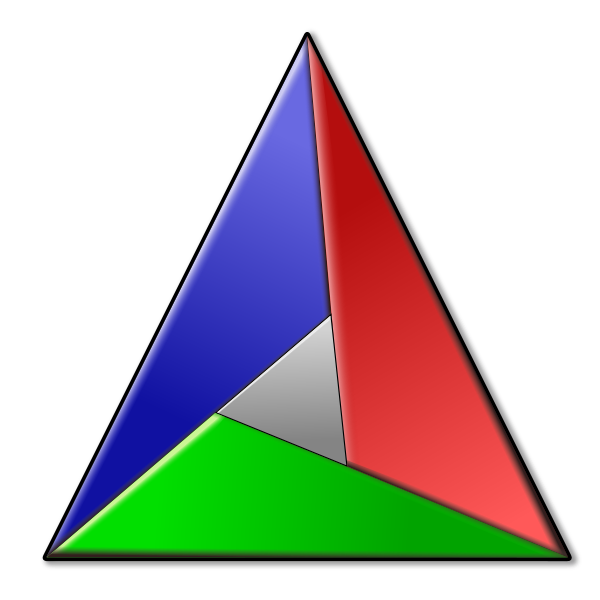
\includegraphics[width=15mm]{images/cmake}}  \textit{\textbf{CMake} est un « moteur de production » multiplate-forme. [...] Il s'occupe de la génération de fichiers de construction standards : makefiles sous Unix, et fichiers de projet Visual Studio sous Windows. Cela permet aux développeurs d'utiliser leur environnement de développement préféré comme à leur habitude.}\footnote{\url{http://fr.wikipedia.org/wiki/Cmake}}

  \vspace{5mm}
Ce logiciel est utilisé pour configurer rapidement et de façon automatique la compilation d'un programme ou d'une bibliothèque.
Il va rechercher lui même les dépendances nécessaires ce qui permet d'avoir les fichiers de projets indépendants de la machine sur laquelle ils sont compiler.

  
\subsection{Doxygen}

\parpic{
\includegraphics[width=25mm]{images/doxygen}}   \textit{\textbf{Doxygen} est un logiciel informatique libre, plus précisément un générateur de documentation, capable de produire une documentation logicielle à partir du code source d'un programme. Pour cela, il tient compte de la grammaire du langage dans lequel est écrit le code source, ainsi que des commentaires s'ils sont écrits dans un format particulier.}\footnote{\url{http://fr.wikipedia.org/wiki/Doxygen}}

  \vspace{5mm}
Lorsqu'on écrit un programme on ajoute souvent des commentaires afin de s'y retrouver facilement.
Doxygen permet de créer, à partir de ces commentaires, un site web regroupant toutes les informations contenues dans le code.
Il supporte un très grand nombre de langages :  C, C++, Java, Objective C, Python, IDL, VHDL et dans une certaine mesure PHP, C\#, D et Fortran.
Via un script, on peut transformer de façon automatique du code MatLab pour qu'il soit compatible avec Doxygen.

\subsection{GDB}

\parpic{
\includegraphics[width=28mm]{images/gdb}}   \textit{\textbf{GNU Debugger}, également appelé gdb, est le débogueur standard du projet GNU. Il est portable sur de nombreux systèmes type Unix et fonctionne pour plusieurs langages de programmation, comme le C, le C++ et le Fortran. Il fut écrit par Richard Stallman en 1988. gdb est un logiciel libre, distribué sous la licence GNU GPL.}\footnote{\url{http://fr.wikipedia.org/wiki/GNU_Debugger}}

  \vspace{5mm}
Pour trouver les erreurs dans un programme, il est plus facile d'utiliser un logiciel qui va nous les localiser plutôt que de les chercher à la main.
GDB permet d'obtenir la ligne, la fonction ou le fichier qui pose problème.

\newpage
\subsection{Qt}

\parpic{
\includegraphics[width=18mm]{images/qt}}   \textit{\textbf{Qt} est :\\
 - une API orientée objet et développée en C++ par Qt Development Frameworks, filiale de Digia. Qt offre des composants d'interface graphique (widgets), d'accès aux données, de connexions réseaux, de gestion des fils d'exécution, d'analyse XML, etc.\\
 - par certains aspects un framework lorsqu'on l'utilise pour concevoir des interfaces graphiques ou que l'on architecture son application en utilisant les mécanismes des signaux et slots par exemple.}
 
    \textit{Qt permet la portabilité des applications qui n'utilisent que ses composants par simple recompilation du code source. Les environnements supportés sont les Unix (dont Linux) qui utilisent le système graphique X Window System ou Wayland, Windows, Mac OS X et également Tizen. Le fait d'être une bibliothèque logicielle multiplate-forme attire un grand nombre de personnes qui ont donc l'occasion de diffuser leurs programmes sur les principaux OS existants.}\footnote{\url{http://fr.wikipedia.org/wiki/Qt}}

\vspace{5mm}
Cette bibliothèque, simple d'utilisation, permet d'accéder rapidement à de nombreuse fonctionnalité (interface graphique, MySQL, XML, network, \dots).
Des exemples pourront être abordés pendant le module.

\end{document}
